\section{Method}
\begin{figure*}[t!]
    \centering
    \begin{subfigure}[t]{0.5\textwidth}
        \centering
        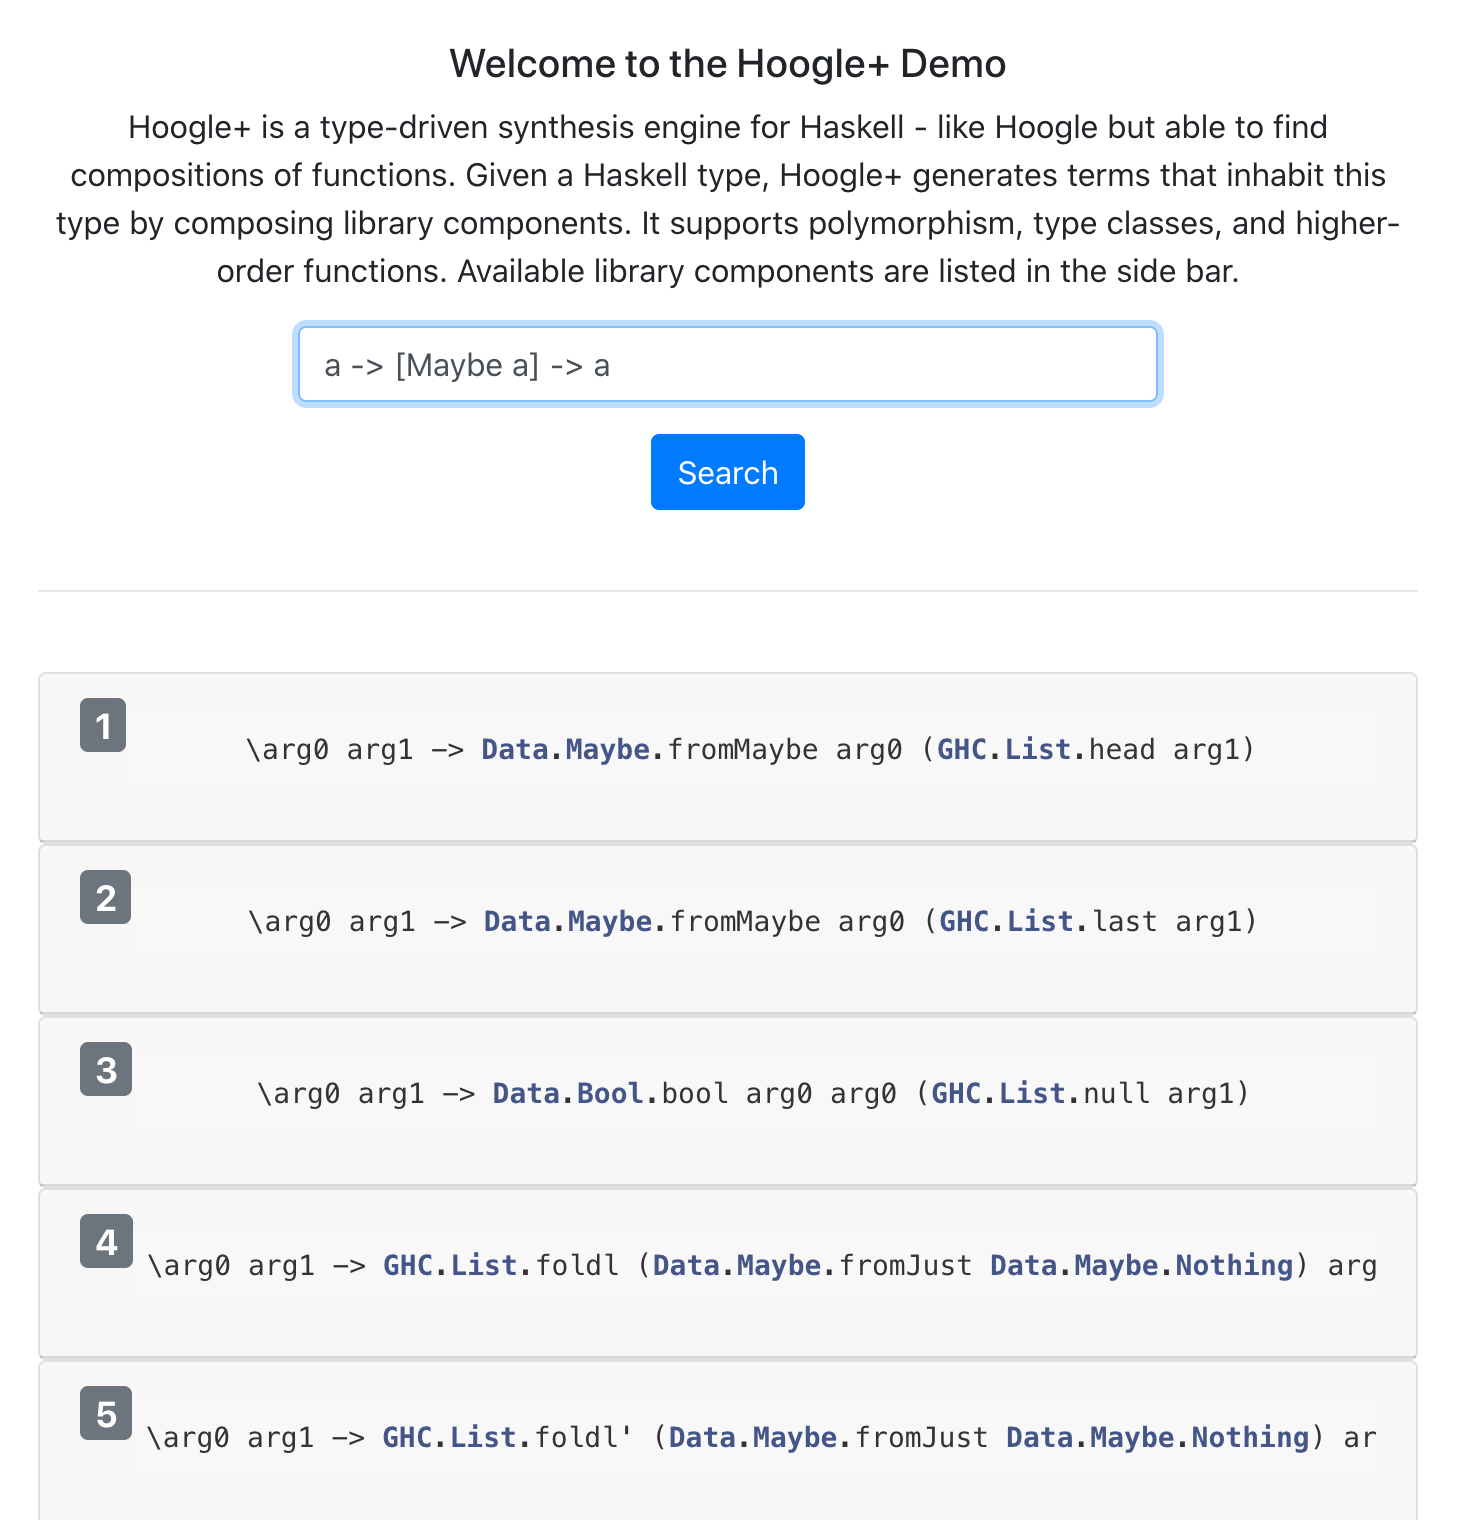
\includegraphics[width=\textwidth]{method/control-ui.png}
        \caption{Control treatment, no examples}
    \end{subfigure}%
    ~
    \begin{subfigure}[t]{0.5\textwidth}
        \centering
        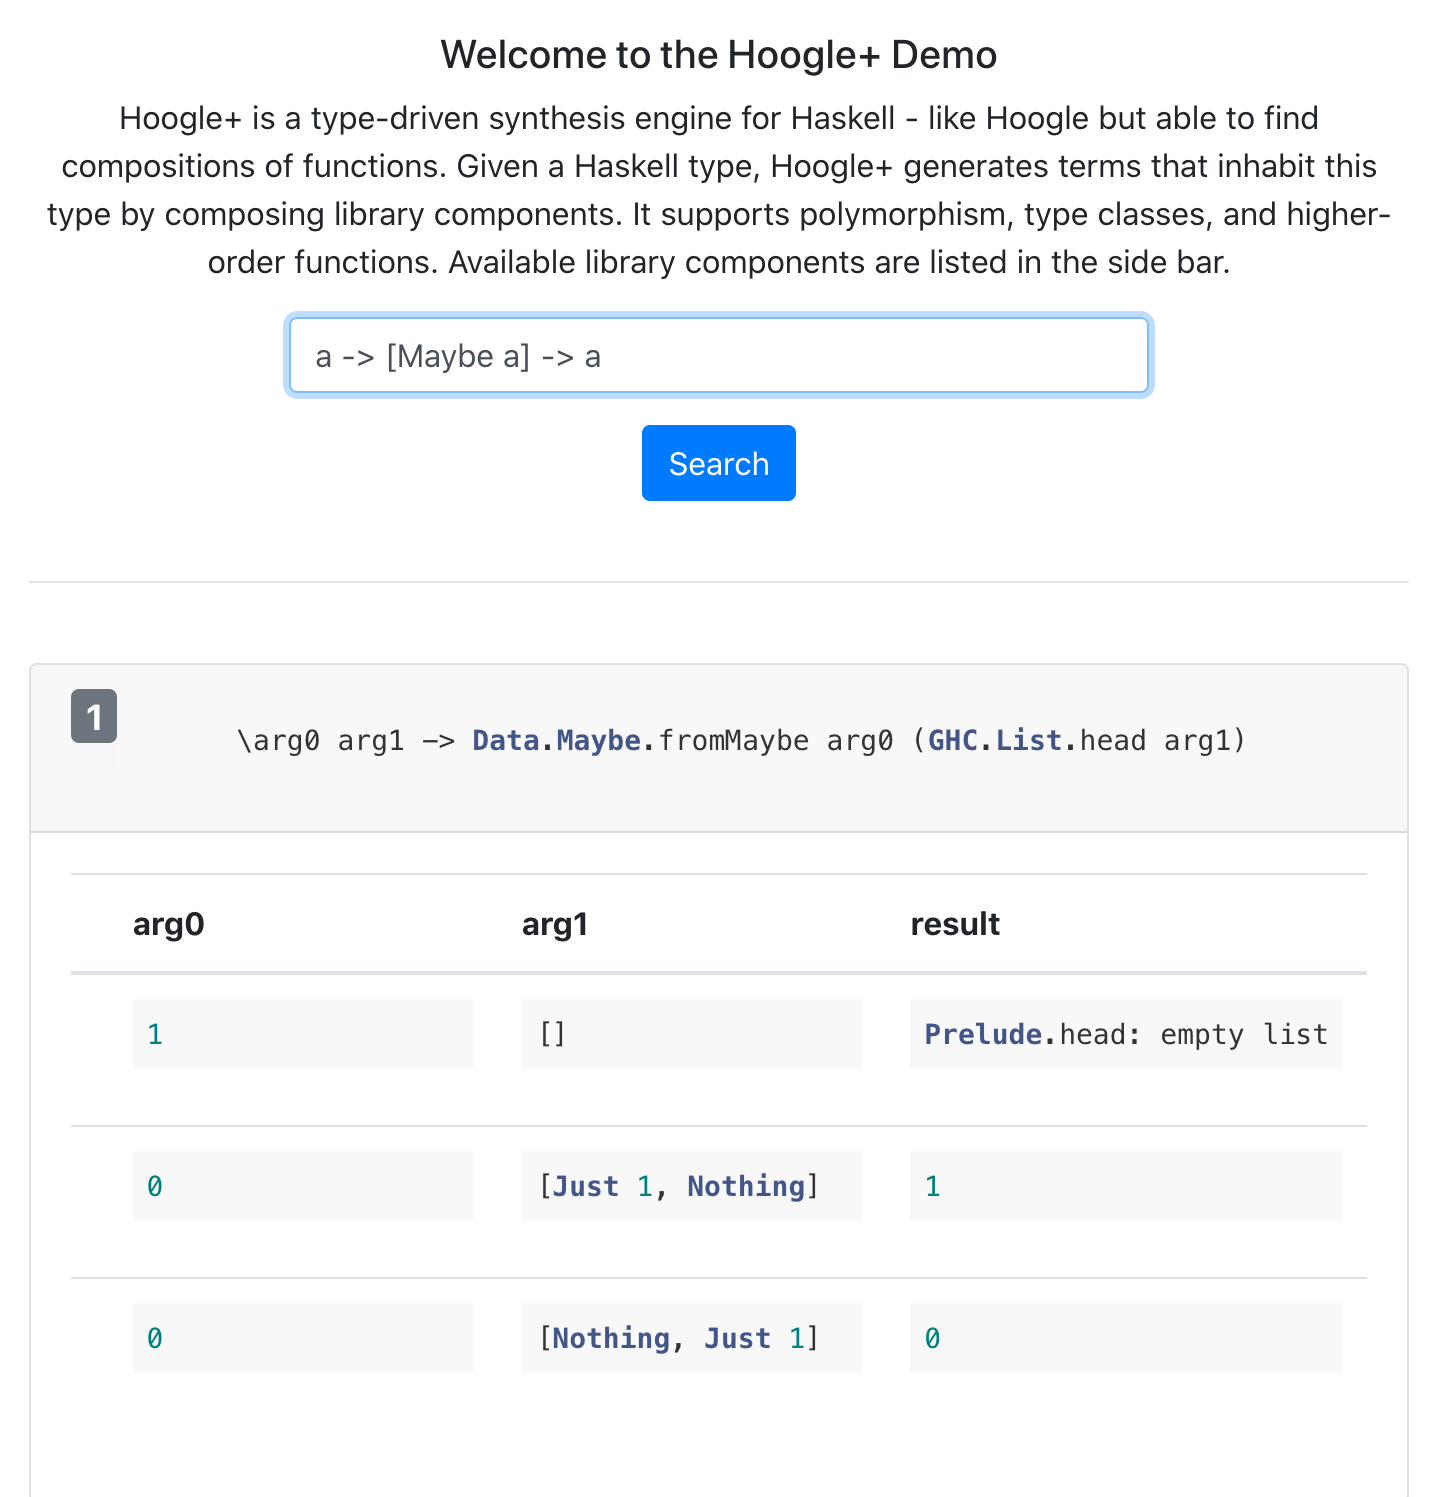
\includegraphics[width=\textwidth]{method/treatment-ui.png}
        \caption{Experimental treatment, examples}
    \end{subfigure}
    \caption{Each participant received one of the two treatments for the duration of the study.}
    \label{fig:ui}
\end{figure*}
To assess whether examples aid recognition of candidate programs, we
developed two variants of a synthesizer interface (see Figure~\ref{fig:ui})

\paragraph{No-examples variant}
%
In the \noexamples variant, a user can enter a Haskell type signature at the top and get a
list of 10 candidate programs back.
%
These candidates are unmodified and in the same order that \hoogleplus
synthesizer generates them.
%
The results are deterministic meaning that for a given type signature, the
response is always the same.

\paragraph{Examples variant}
The \examples variant extends the \noexamples variant with input/output
examples for each candidate.
%
For each, type signature in the study, we manually created three simple
inputs of the appropriate type.
%
Each candidate program received the same three inputs.


\subsection{Procedure}
We gathered 10 haskell-literate participants from around our department's
building and from the local Hillcrest community.
%
Participants were each assigned to either the \noexamples treatment or the
\examples treatment for the duration of the study.
%
Each participant was presented a laptop with their respective tool variant open
and an interactive haskell interpreter (GHCI) open to the side.
%
Throughout the study participants were allowed to use only the tool and the
interpreter.

After a brief tutorial tasks, participants were asked to complete 4 tasks.
%
Each task consisted of a type signature they would enter, and an informal
english description of the behavior they were looking for.
%
They would then enter the type signature and identify the candidate program that
met the specification, if it was present.
%
Participants were told at the beginning that the solution may not be present
in the list---Task 3 did not have a solution in the list.

After completing the four tasks, the candidates were given a brief survey
that asked them about their haskell experience, their opinions on the tool,
and their strategies for finding the correct answer.


\subsection{Measures}

For each participant, we measured:
\begin{itemize}
    \item Time-to-correct solution (per task)
    \item Count of incorrect selections (per task)
    \item Count and type of interpreter queries (across all tasks)
\end{itemize}

The first metric directly tests the hypothesis that examples improve
selection speed, but the result could be misleading if there was also a
change in selection accuracy.
%
Counting incorrect guesses ensures that any such change is captured.
%
Beyond assessing the effectiveness of examples, measuring how often and why
participants used the interactive interpreter provides insight into any
behavior changes that might occur.
